\section{Atividades}

\subsection{Atividade -- Ataque de CSRF com Alteração de Senha e Logout}

\paragraph{}
Foi realizada a análise da funcionalidade de alteração de senha da aplicação
\texttt{vulneravel.com}, identificando a ausência de mecanismos de proteção
contra ataques Cross-Site Request Forgery (CSRF).

\paragraph{}
Com base nos parâmetros utilizados pelo formulário da aplicação, foi criada uma
página maliciosa contendo requisições capazes de alterar a senha do usuário
autenticado e, em seguida, encerrar sua sessão ativa.

\paragraph{}
Ao acessar a página hospedada em um domínio externo, o navegador enviou
automaticamente as requisições utilizando os cookies de sessão da vítima,
resultando na alteração da senha e na execução do logout sem qualquer
confirmação adicional.

\paragraph{}
Para validar a exploração da vulnerabilidade, foi utilizada a aba
\textit{Network} das Ferramentas de Desenvolvedor do navegador, permitindo
visualizar as requisições enviadas para a aplicação vulnerável.

\begin{figure}[H]
    \centering
    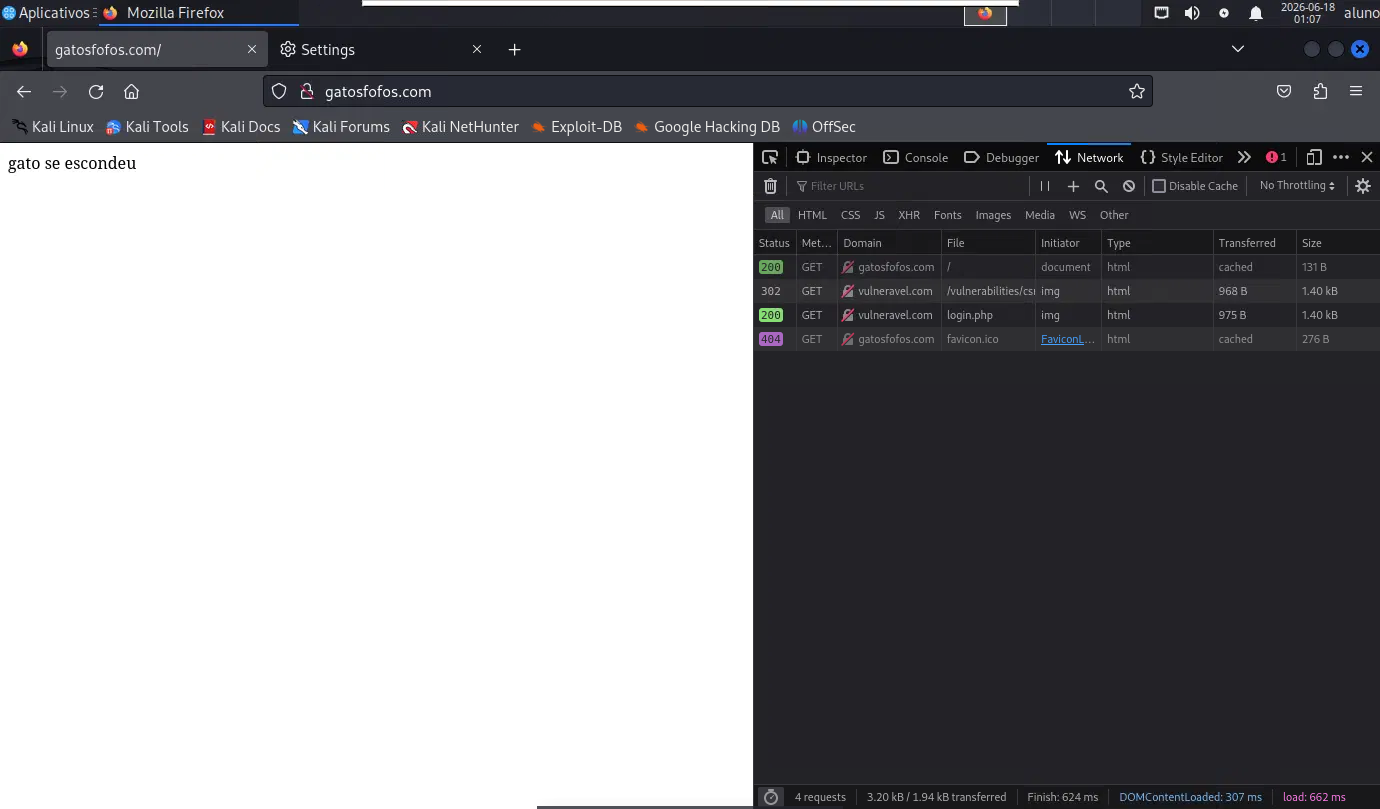
\includegraphics[width=0.95\textwidth]{./fig/network-csrf.png}
    \caption{Janela Network exibindo as requisições responsáveis pela alteração
    da senha e pelo encerramento da sessão do usuário.}
\end{figure}

\paragraph{}
A captura demonstra o envio bem-sucedido das requisições CSRF executadas pelo
navegador da vítima, confirmando a execução do ataque.

\paragraph{}
Como evidência adicional, foi realizado um novo processo de autenticação
utilizando a senha originalmente configurada para a conta.

\begin{figure}[H]
    \centering
    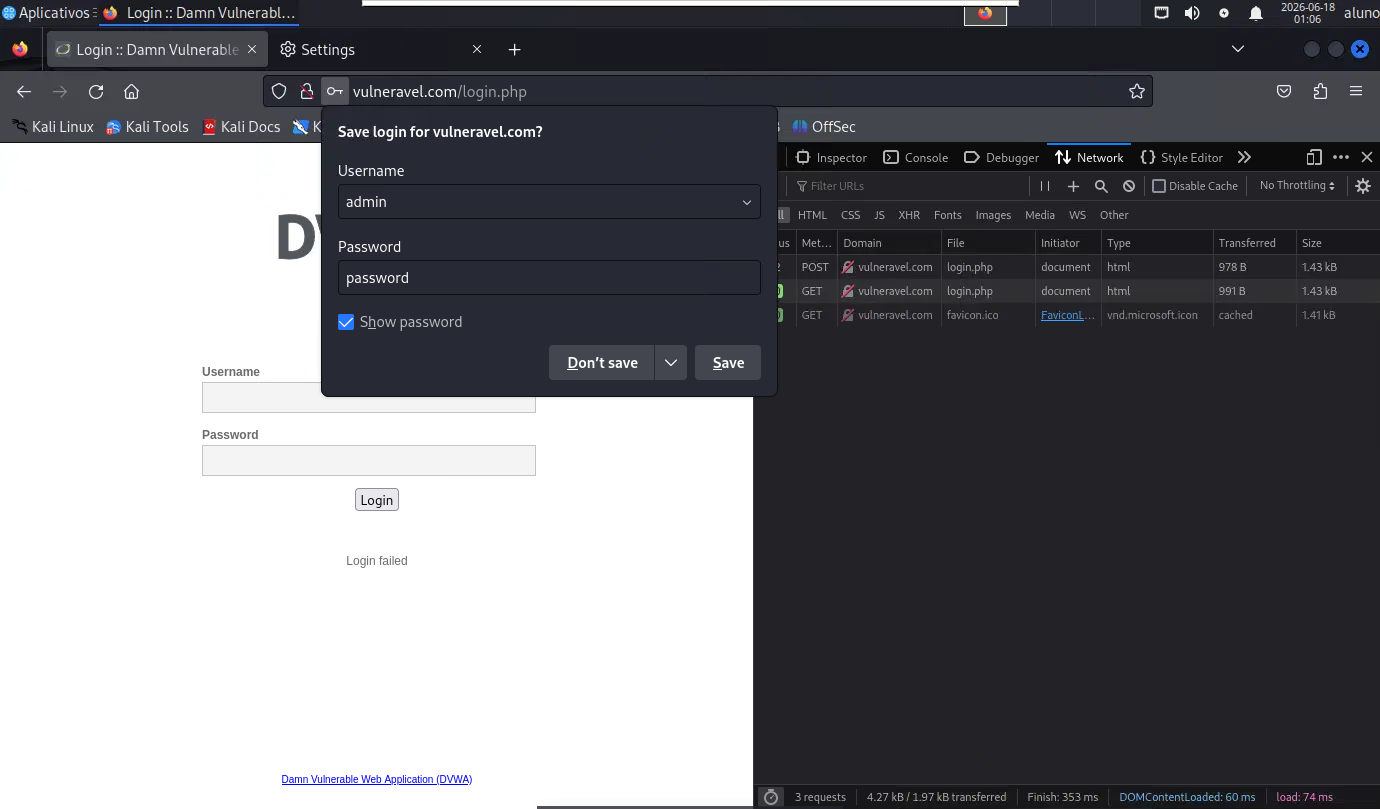
\includegraphics[width=0.95\textwidth]{./fig/login-falha.png}
    \caption{Falha de autenticação utilizando a senha original da conta após a
    execução do ataque CSRF.}
\end{figure}

\paragraph{}
A impossibilidade de autenticação com a senha anterior comprova que a
requisição forjada alterou com sucesso a credencial da vítima. Dessa forma,
fica evidenciado que o ataque CSRF foi capaz de modificar informações
sensíveis da conta e encerrar a sessão do usuário sem seu consentimento.
